\documentclass{standalone}
\usepackage{tikz}
\usepackage{pgfplots}
\pgfplotsset{width=32cm,height=18cm,compat=1.3}
\pgfplotsset{every tick label/.append style={font=\Huge}}
\usepackage{filecontents}

\usetikzlibrary{patterns}

\definecolor{citrine}{rgb}{0.89, 0.82, 0.04}

\begin{document}
	\centering
		\vspace{1.5em}
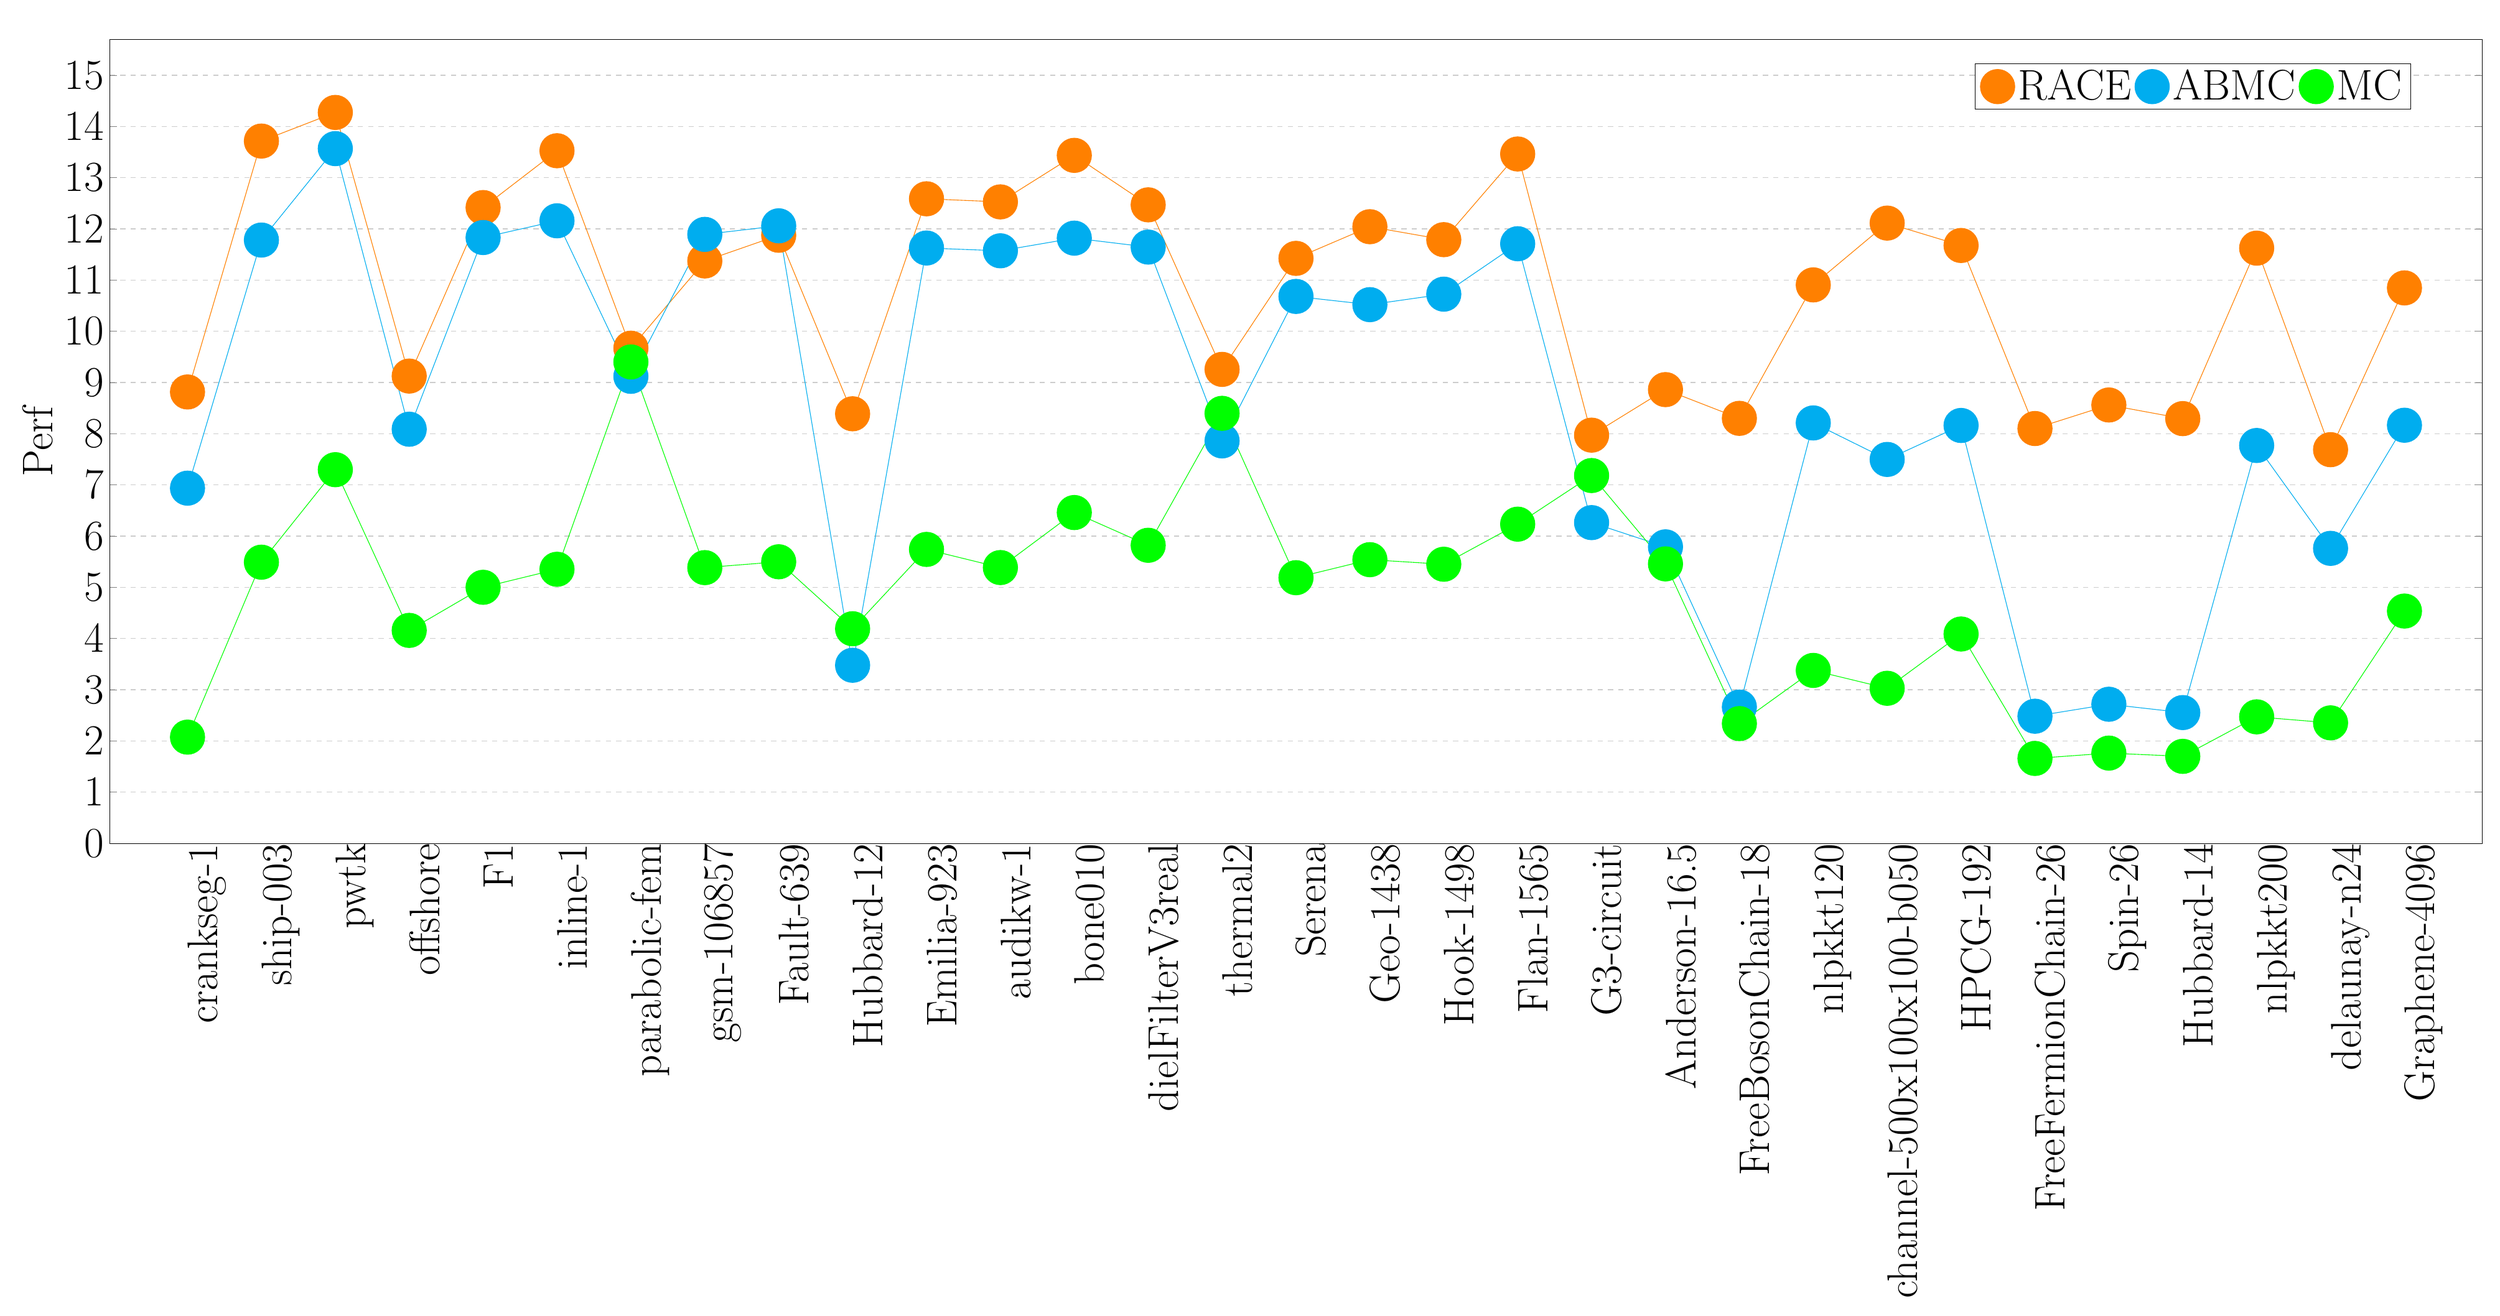
\begin{tikzpicture}
		%	\node at (13.25,15) {\LARGE{}};
			\begin{axis}[
		%	xmin=0.25, xmax=7.25,
			ymin=0, %ymax=3.25,
			xtick={1, 2, 3, 4, 5, 6, 7, 8, 9, 10, 11, 12, 13, 14, 15, 16, 17, 18, 19, 20, 21, 22, 23, 24, 25, 26, 27, 28, 29, 30, 31},
		%	ytick={0,0.5,1,1.5,2,2.5,3},
			xticklabels={crankseg-1, ship-003, pwtk, offshore, F1, inline-1, parabolic-fem, gsm-106857, Fault-639, Hubbard-12, Emilia-923, audikw-1, bone010, dielFilterV3real, thermal2, Serena, Geo-1438, Hook-1498, Flan-1565, G3-circuit, Anderson-16.5, FreeBosonChain-18, nlpkkt120, channel-500x100x100-b050, HPCG-192, FreeFermionChain-26, Spin-26, Hubbard-14, nlpkkt200, delaunay-n24, Graphene-4096},
			width  = 50cm,
			height = 18cm,
			major x tick style = transparent,
			%	minor ytick={1, 5, 10, 15, 20, 25, 30 ,35,40},
			grid = minor,	
			%add_bar_commands
			ymajorgrids = true,
			grid style={dashed, gray!40},
			ylabel = {\Huge{Perf}},
		%	symbolic x coords={Graphene-2048-2048, Graphene-4096-4096, Spin-24-24-24},
			x tick label style={rotate=90, anchor=north east, inner sep=0mm, font={\Huge}},
			tick label style={font={\Huge}},
			scaled y ticks = false,
			enlarge x limits=0.035,
			legend cell align=left,
			legend style={font=\Huge},
			legend columns=-1,
			legend style={
				%at={(1,1.05)},
				%anchor=south east,
				%column sep=1ex,
				legend pos=north east
			},
			%spl_legend_code
			title= {\Huge\scalebox{1.5}{{}}}
			]

\addplot[ mark=*, mark size=10pt, mark options={orange}, draw=orange ] plot coordinates{(1,8.814827) (2,13.714179) (3,14.273255) (4,9.125201) (5,12.416125) (6,13.525165) (7,9.669759) (8,11.372827) (9,11.874714) (10,8.388622) (11,12.586951) (12,12.526642) (13,13.435144) (14,12.468738) (15,9.255635) (16,11.423776) (17,12.041858) (18,11.788976) (19,13.462140) (20,7.971574) (21,8.860685) (22,8.299701) (23,10.905698) (24,12.112548) (25,11.675337) (26,8.101027) (27,8.560665) (28,8.294585) (29,11.623303) (30,7.687837) (31,10.846834)};
\addplot[ mark=*, mark size=10pt, mark options={cyan}, draw=cyan ] plot coordinates{(1,6.936365) (2,11.781336) (3,13.566779) (4,8.087444) (5,11.830486) (6,12.157100) (7,9.120319) (8,11.892110) (9,12.059205) (10,3.478216) (11,11.625918) (12,11.571445) (13,11.818585) (14,11.644027) (15,7.859110) (16,10.680561) (17,10.519765) (18,10.724788) (19,11.709422) (20,6.263598) (21,5.790380) (22,2.661792) (23,8.210047) (24,7.497267) (25,8.160697) (26,2.482975) (27,2.716768) (28,2.554161) (29,7.769786) (30,5.760882) (31,8.165374)};
\addplot[ mark=*, mark size=10pt, mark options={green}, draw=green ] plot coordinates{(1,2.074471) (2,5.491078) (3,7.297117) (4,4.159082) (5,5.000604) (6,5.352471) (7,9.401340) (8,5.384840) (9,5.498699) (10,4.191218) (11,5.740404) (12,5.386030) (13,6.460395) (14,5.820991) (15,8.397550) (16,5.187995) (17,5.539975) (18,5.450630) (19,6.233426) (20,7.182862) (21,5.457603) (22,2.338942) (23,3.377477) (24,3.028531) (25,4.088213) (26,1.658420) (27,1.762873) (28,1.699188) (29,2.470589) (30,2.353157) (31,4.536472)};
	%addplot cmd

	\legend{RACE, ABMC, MC}

	\end{axis}			
\end{tikzpicture}

\end{document}

